
\begin{textblock}{16}(0,2)
\begin{figure}
    \centering
    \begin{tikzpicture}

\node<1->[inner sep=0pt] (motherboard) at (3,0)
    {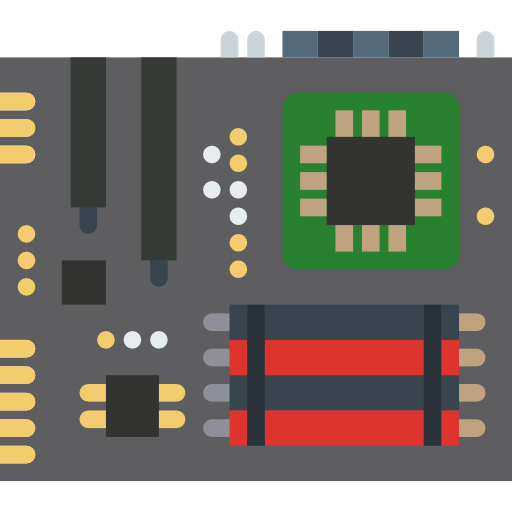
\includegraphics[width=.12\textwidth]{Simulation_sayem/pictures/motherboard.png}};  
\node<1->[inner sep=0pt] (videocard) at (3,3)
    {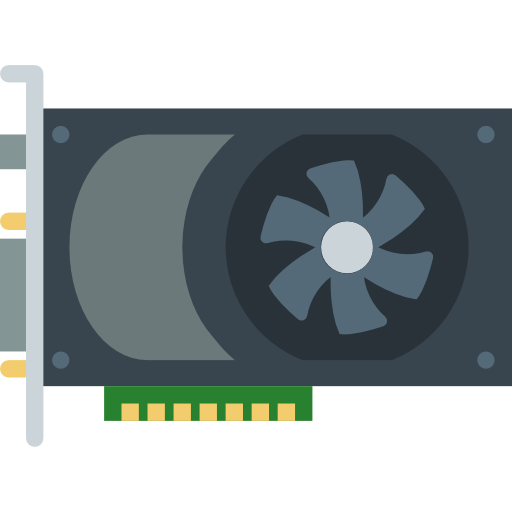
\includegraphics[width=.12\textwidth]{Simulation_sayem/pictures/video-card.png}};
    
\node<1->[inner sep=0pt] (memory) at (0,0)
    {
\includegraphics[width=.12\textwidth]{Simulation_sayem/pictures/memory.png}};
    
\node<1->[inner sep=0pt] (casing) at (6,0)
    {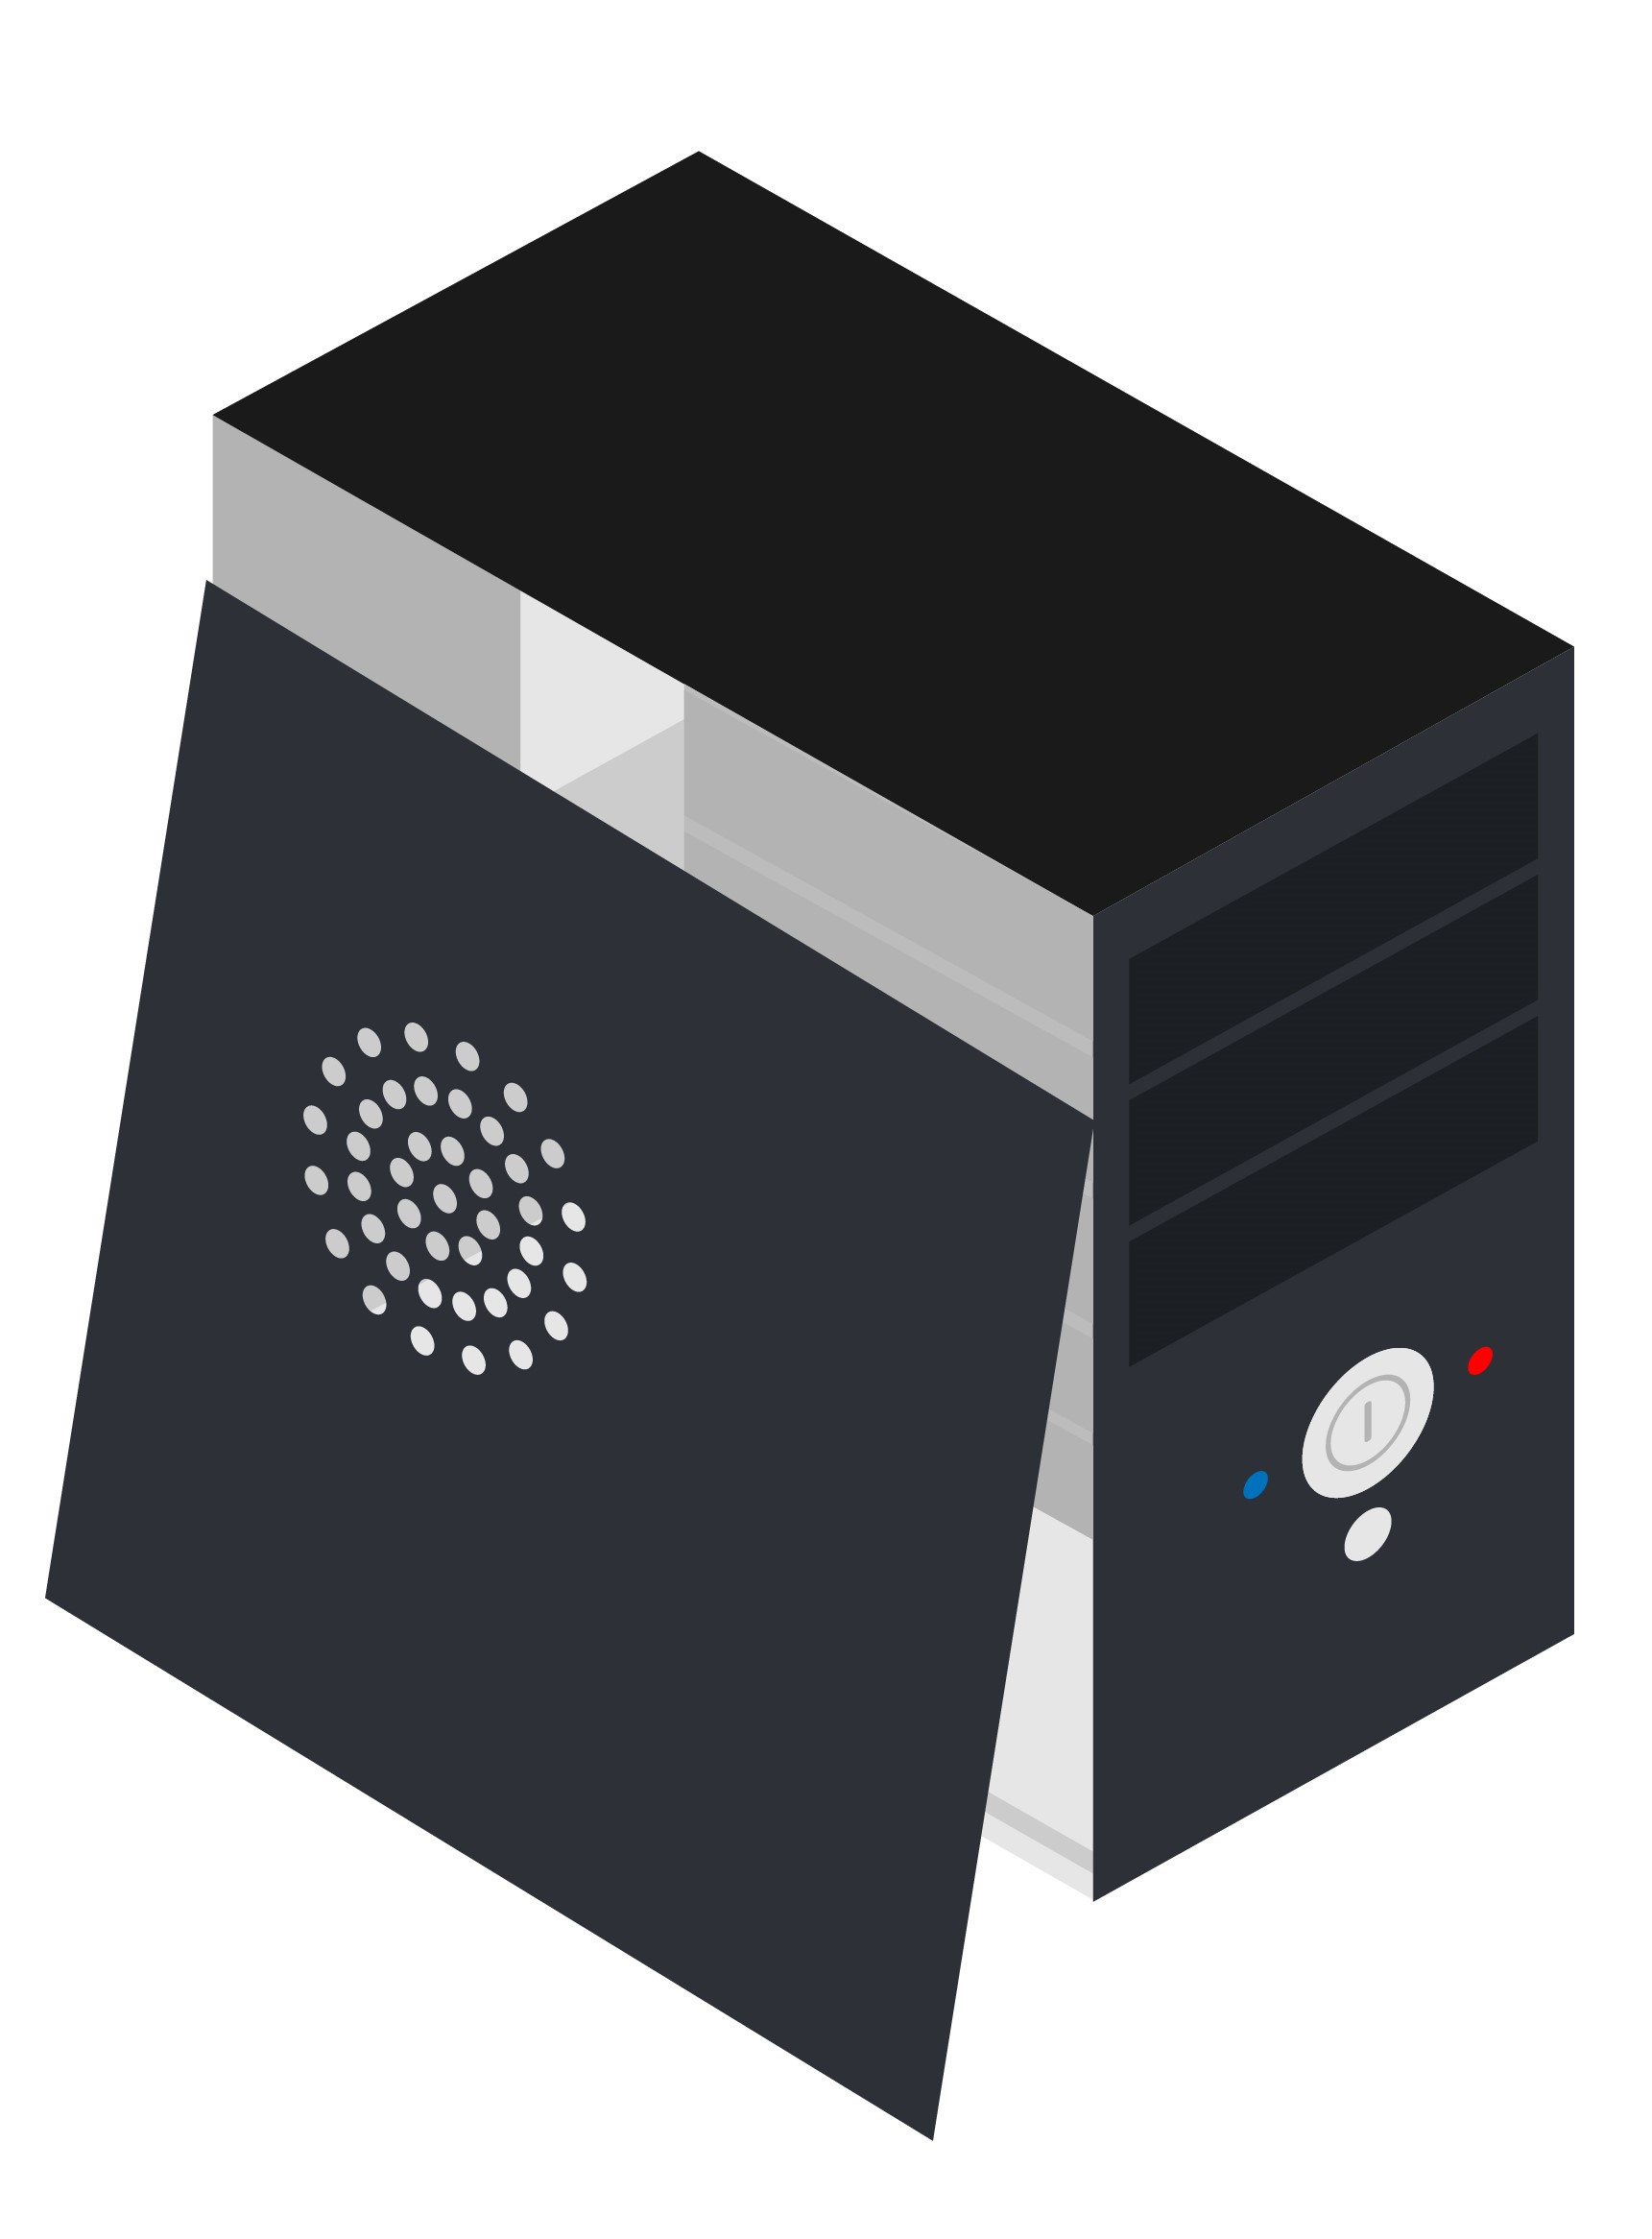
\includegraphics[width=.12\textwidth]{Simulation_sayem/pictures/casing.jpg}};
\node<1->[inner sep=0pt] (PSU) at (6,3)
    {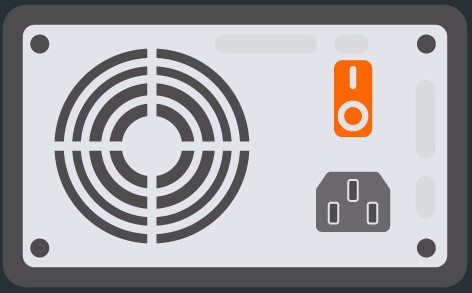
\includegraphics[width=.12\textwidth]{Simulation_sayem/pictures/powerSupply.jpg}};
\node<1->[inner sep=0pt] (CPU) at (0,3)
    {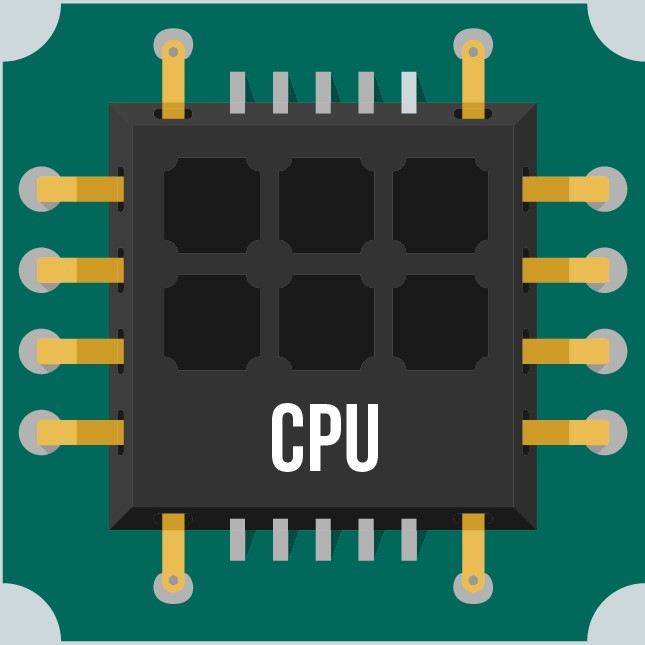
\includegraphics[width=.08\textwidth]{Simulation_sayem/pictures/processor.jpg}};


\node<2->[inner sep=0pt] (motherboardtik) at (3,0)
    {
\includegraphics[width=.09\textwidth]{Simulation_sayem/pictures/tik.png}};
\node<3->[inner sep=0pt] (CPUtik) at (0,3)
    {
\includegraphics[width=.09\textwidth]{Simulation_sayem/pictures/tik.png}};
\node<4->[inner sep=0pt] (videocardtik) at (3,3)
    {
\includegraphics[width=.09\textwidth]{Simulation_sayem/pictures/tik.png}};
\node<5->[inner sep=0pt] (PSUtik) at (6,3)
    {
\includegraphics[width=.09\textwidth]{Simulation_sayem/pictures/tik.png}};
\node<6->[inner sep=0pt] (casingtik) at (6,0)
    {
\includegraphics[width=.09\textwidth]{Simulation_sayem/pictures/tik.png}};
\node<7->[inner sep=0pt] (memorytik) at (0,0)
    {
\includegraphics[width=.09\textwidth]{Simulation_sayem/pictures/tik.png}};

\draw<1-> [inactive edge] (videocard) --(PSU);
\draw<1-> [inactive edge] (motherboard) --(videocard);
\draw<1-> [inactive edge] (CPU) --(videocard);
\draw<1-> [inactive edge] (motherboard) --(CPU);
\draw<1-> [inactive edge] (PSU) --(casing);
\draw<1-> [inactive edge] (motherboard) --(casing);
\draw<1-> [inactive edge] (motherboard) --(memory);


\end{tikzpicture}
\end{figure}
\end{textblock}


\begin{textblock}{14}(1,11)
    \begin{itemize}
        \item<2-> Our shopping list
    \end{itemize}
\end{textblock}


\begin{textblock}{14}(2.5,12)
    
    
    \begin{tikzpicture}

\node<2->[inner sep=0pt] (motherboard) at (0,0)
    {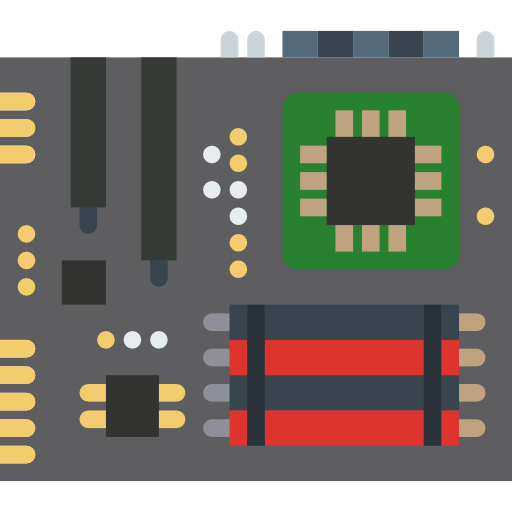
\includegraphics[width=.10\textwidth]{Simulation_sayem/pictures/motherboard.png}};  
\node<4->[inner sep=0pt] (videocard) at (4,0)
    {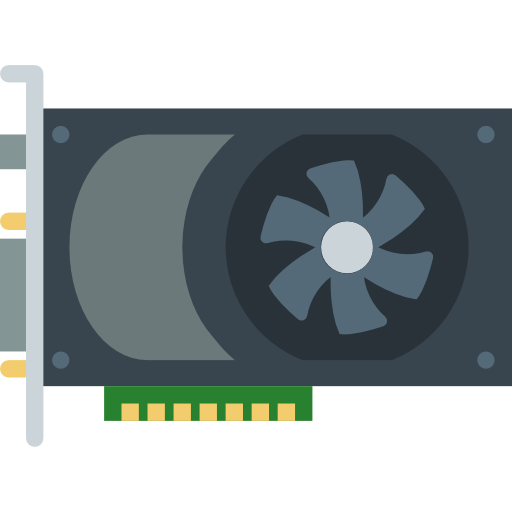
\includegraphics[width=.10\textwidth]{Simulation_sayem/pictures/video-card.png}};
    
\node<7->[inner sep=0pt] (memory) at (10,0)
    {
\includegraphics[width=.10\textwidth]{Simulation_sayem/pictures/memory.png}};
    
\node<6->[inner sep=0pt] (casing) at (8,0)
    {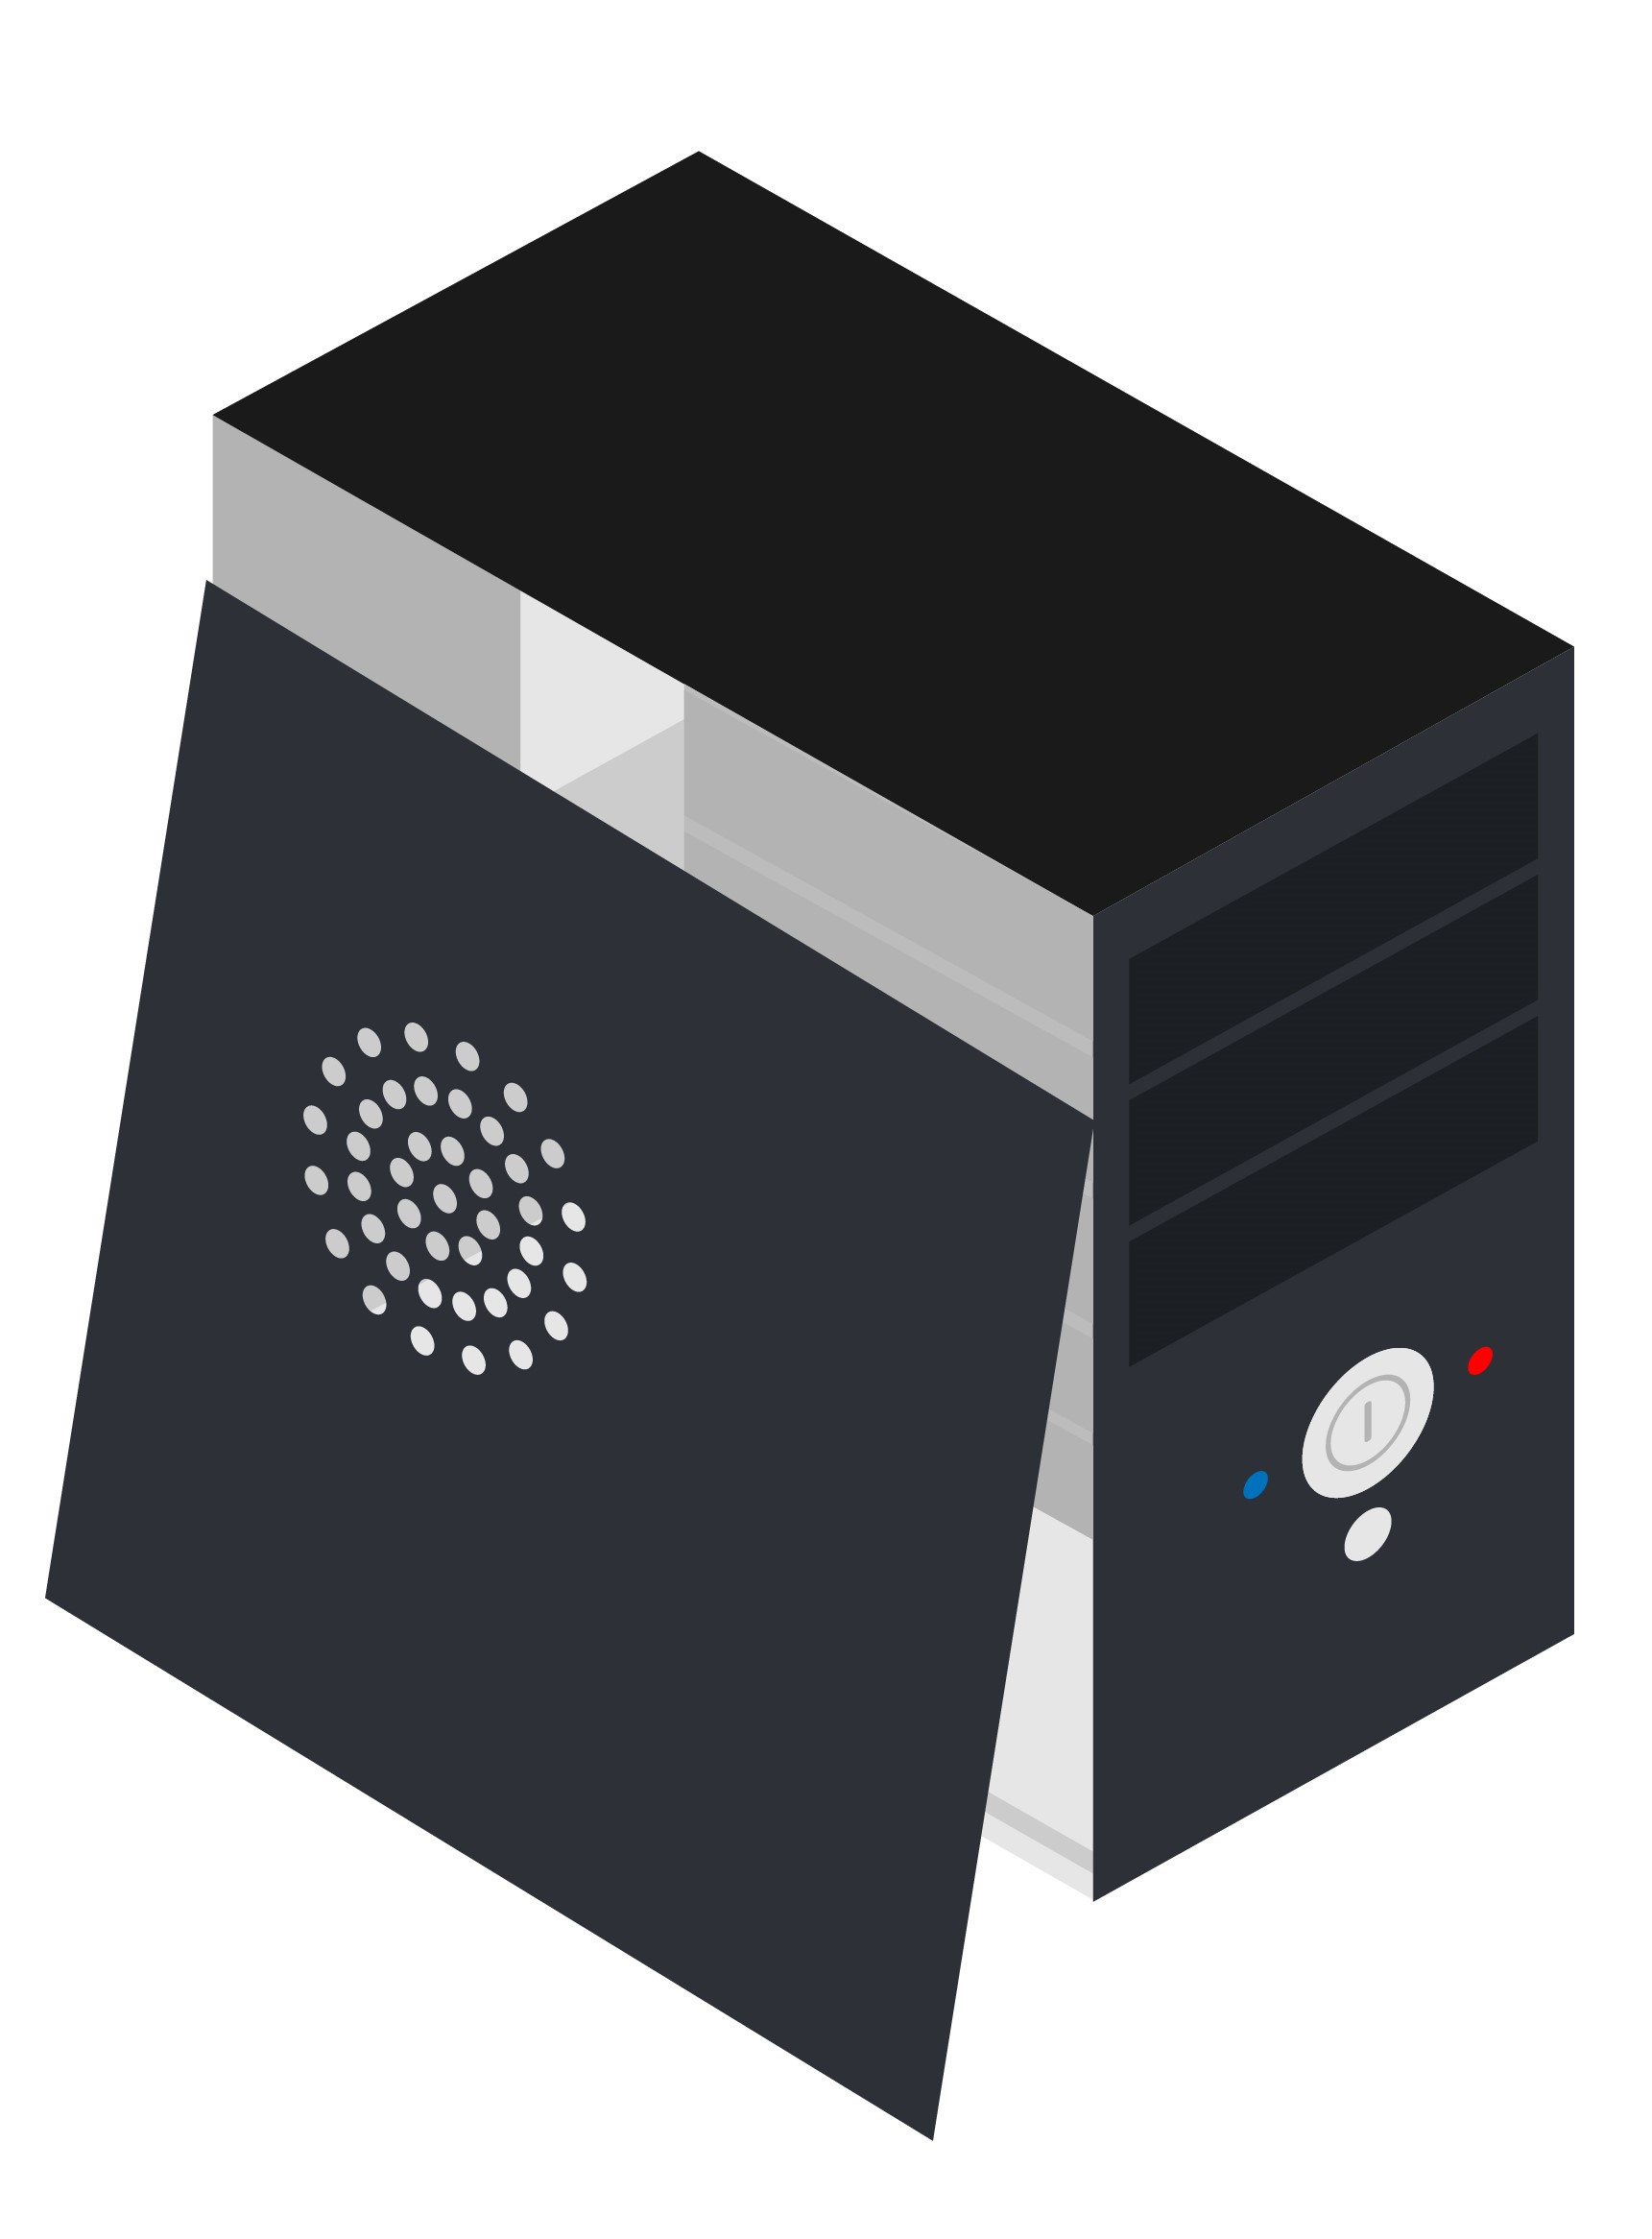
\includegraphics[width=.073\textwidth]{Simulation_sayem/pictures/casing.jpg}};
\node<5->[inner sep=0pt] (PSU) at (6,0)
    {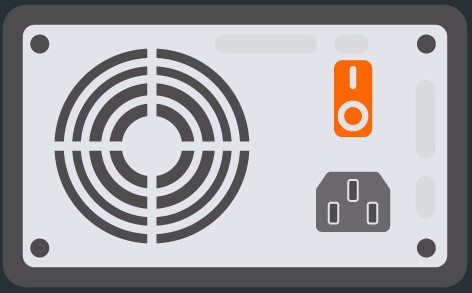
\includegraphics[width=.10\textwidth]{Simulation_sayem/pictures/powerSupply.jpg}};
\node<3->[inner sep=0pt] (CPU) at (2,0)
    {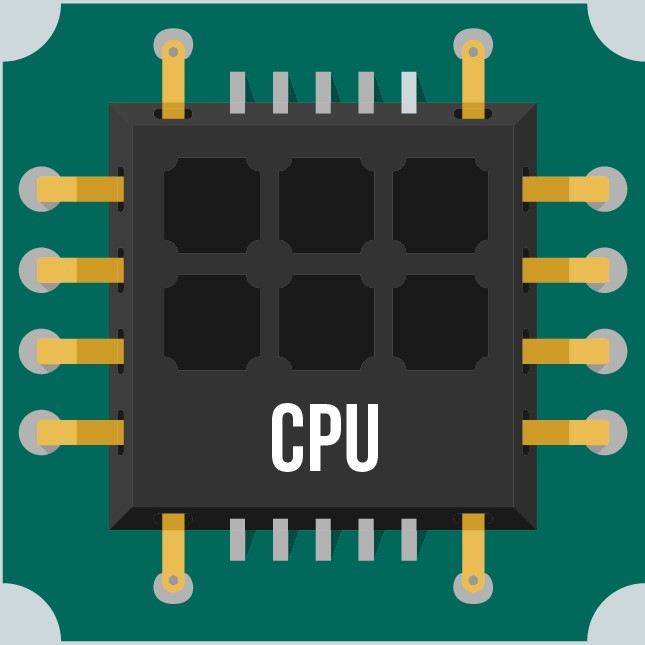
\includegraphics[width=.06\textwidth]{Simulation_sayem/pictures/processor.jpg}};



\end{tikzpicture}

\end{textblock}